\documentclass{article}

\title{Countdown: The Numbers Behind Letters}
\author{Alex Room}
\date{\today}

\usepackage{minted}
\usepackage[numbers,sort]{natbib}
\usepackage{graphicx}
\usepackage{caption}
\usepackage{subcaption}

\begin{document}

\maketitle

Channel 4's TV show Countdown consists of two rounds; a numbers round, where players take turns to choose a set of 6 numbers (from their choice number of 'large' and 'small' numbers), then must use them (but only once each) with basic arithmetic to equal a randomly generated number. The letters round, meanwhile, has players choose random vowels and consonants to form a board of 9 letters, and then must find the longest word they can create from these letters. The former has been extensively studied; even so far as solved \citep{ColtonCountdown}, whereas the letters round is much less so. In this paper, we simulate rounds of Countdown's letters round in order to statistically analyse the largest words possible; in particular, which number of vowels is ideal to have room for the largest words (and thus the most points)?

We begin by turning a dictionary file into a set. For this paper, I used the SOWPODS scrabble words dictionary; this is simply as this dictionary doesn't contain proper nouns, pre/suffixes, and other words not allowed in Countdown.
\begin{minted}{python}
with open('sowpods.txt', 'r') as Words:
    string = Words.read()
    sowpods = (string.split('\n'))
    sowpods.remove('')
    sowpods = {str(i) for i in sowpods if len(i) <= 9}
#converts the SOWPODS scrabble dictionary into a set
\end{minted}

To check this dictionary against our board, we turn the board into a power set\footnote{Apart from reversing the order of the sets, this is identical to the power set function in https://docs.python.org/3/library/itertools.html#itertools-recipes}; that is, create a set of every possible combination of letters (word or not). Here we sort them from longest to shortest - we are finding the longest word possible on each board, so there's no use checking 36 (${9\choose\\2}$) 2-letter sets if there are eligible 7-letter sets. This allows us to compare these strings created from the board against those in the dictionary in the form of tuples.
\begin{minted}{python}
def powerset(iterable):
    '''powerset([1,2,3]) -->  (1,2,3) (1,2) (1,3) (2,3) (1,) (2,) (3,) ()'''
    s = list(iterable)
    return itertools.chain.from_iterable(itertools.combinations(s, r)
                                         for r in range(len(s)+1, 1, -1))
\end{minted}

We then can use this dictionary and definition to create our solve\_board function, which creates a countdown board with a given number of vowels and finds the longest word that can be created from it. The variables 'vowels' and 'consonants' are the obvious strings.
\begin{minted}{python}

#turning the dictionary into a set of split letters, each word as a tuple
dictionary = set([tuple(sorted(word)) for word in sowpods])

def solve_board(vowel_number, 
                display_board=False,
                dictionary=dictionary,
                vowels=vowels,
                consonants=consonants):
    '''creates a countdown board of 9 letters and returns the largest word present'''
    board = []
    length = [0]

    #randomly generates the board
    board = list(np.random.choice(list(vowels), vowel_number, replace=True))
    board += list(np.random.choice(list(consonants), 9 - vowel_number, replace=True))
    if display_board is True:
        print(board)
            
    #checks for words that can be created using the board letters,
    #returns the maximum word length possible
    sorted_board = tuple(sorted(board))
    for subset in powerset(sorted_board):
        if subset in dictionary:
            return subset
    return ([])
\end{minted}

Finally, this function is iterated over a large number of repetitions to find the average longest word for each vowel number.
\begin{minted}{python}
averages = []
for v in range (0, 10):
    highest = [] 
    for _ in range (0, 50000):
        highest.append(len(solve_board(v)))        
    averages.append(sum(highest) / len(highest))
\end{minted}

\newpage

Graphing the average word length for each vowel number, we get a curve like so:

\begin{center}
    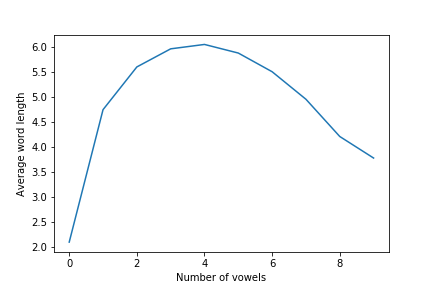
\includegraphics[width=.4\textwidth]{english.png}
\end{center}


This would suggest that the ideal number of vowels on the board is 3-4, although the consequences of choosing extremely high vowel numbers are less than those of choosing zero or one.

As further analysis, Countdown is inspired by French TV show \textit{Des chiffres et des lettres}, which holds a similar letters round system, but a board of 10 letters is used instead. 

\begin{figure}[!h]
  \begin{subfigure}[b]{0.4\textwidth}
    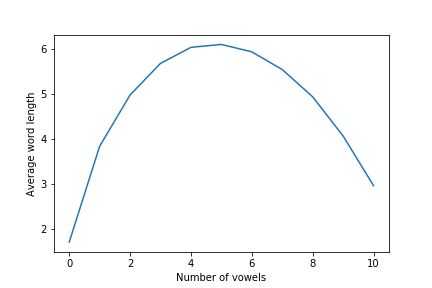
\includegraphics[width=\textwidth]{francais.png}
    \caption{The curve for French words}
    \label{fig:f2}
  \end{subfigure}
  \hfill
  \begin{subfigure}[b]{0.4\textwidth}
    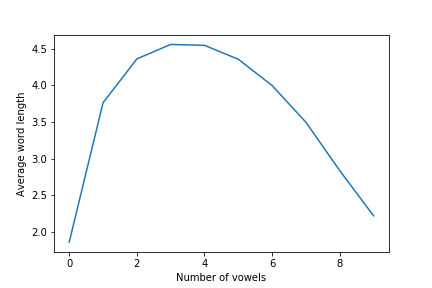
\includegraphics[width=\textwidth]{deutsch.png}
    \caption{The curve for German words}
    \label{fig:f3}
  \end{subfigure}
\end{figure}

Similarly simulating French boards of 10 letters, we find a similar curve, with 4-5 vowels as the peak; this shows similarity in Latin languages, where the length of words and use of specific letters and phonemes stays similar regardless of language due to Zipf's principle of least effort \citep{ZipfHuman}. We do this again for German; although the shape is again similar, peaking at 3-4, the average word length is much lower (a peak of 4.56 versus French's 6.04); Countdown or an equivalent game has not yet reached German television, and this clash between the game's format and the German language may be at least partially at fault. 

\bibliography{bibliography}{}
\bibliographystyle{unsrtnat}

\end{document}

